\definecolor{exxetagray}{gray}{0.75}
\definecolor{itemcolor}{RGB}{179,217,255}
\definecolor{usercolor}{RGB}{255,204,179}

\shorthandoff{"}
\chapter{Methodik und Konzeption}
\label{ch:methodik}
Das folgende Kapitel beschreibt das methodische Vorgehen zur Beantwortung der Forschungsfrage der vorliegenden Arbeit.
Hierfür wird zu Beginn das Kernproblem des Anwendungsfalls identifiziert und in den Gesamtkontext eingebettet.
Darauf folgt eine Beschreibung der durchgeführten quantitativen Forschung.
Abschließend wird die Konzeption des bilateralen Algorithmus beschrieben und der Aufbau des Gesamtsystems vorgestellt.

\section{Problemanalyse}
% Erklärung der genauen Problematik in unserem Anwendungsfall

% \subsection{Probleminterpretation}
% Nutzer = Manager, deren Anforderungen als Vektor dargestellt werden

\section{Art und Ablauf der Forschung}
Um die Forschungsfrage der vorliegenden Arbeit zu beantworten, wurde eine quantitative Forschung in dem IT-Beratungsunternehmen EXXETA durchgeführt.
Der Ablauf der Forschung kann in 4 Stufen unterteilt werden und ist nachfolgend in Abbildung \ref{fig:methodik:abb1} grafisch dargestellt.

\begin{figure}[H]
    \centering
	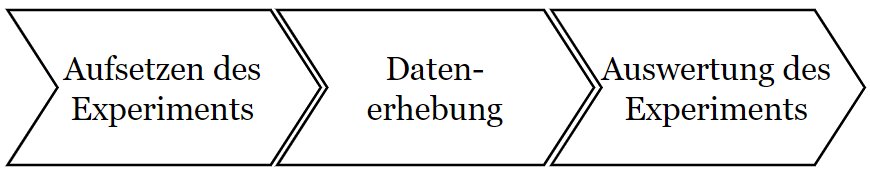
\includegraphics[width=0.95\textwidth]{gfx/prozess-forschung.png}
	\caption[Ablauf der Forschung]{Ablauf der Forschung}
	\label{fig:methodik:abb1}
\end{figure}

Die einzelnen Stufen werden anschließend im Detail erläutert.

\subsection{Aufsetzen der Fallstudie}
Für das Aufsetzen der Fallstudie wurden zu Beginn durch einen Manager des Fachbereichs Java Enterprise Solutions fünf Beispielprojekte mit angeforderten Projektpositionen erstellt.
Nach Angaben des Managers gelten die Beispielprojekte als repräsentativ für häufige Kundenanfragen an den Bereich.
Die Projekte sind in Abbildung \ref{fig:methodik:abb2} dargestellt.

% \begin{table}[htbp]
%     \begin{center}
%     \begin{tabular}{c|c}
%     {\textbf{Fähigkeit}} & {\textbf{Anforderungsniveau}}\\
%     \hline
%     Android & Fortgeschritten \\
%     \hline
% 	Architektur & Fortgeschritten \\
%     \hline
%     Kotlin & Fortgeschritten \\
%     \hline
% 	Mockito & Grundkenntnisse \\
%     \hline
% 	JSON & Grundkenntnisse \\
%     \hline
% 	REST & Grundkenntnisse \\
%     \end{tabular}
%     \end{center}
%     \caption[Beispielprojekte]{Beispielprojekte}
% 	\label{tab:methodik:tab1}
% \end{table}

\begin{figure}[H]
    \centering
    \subfloat[Projekt 1]{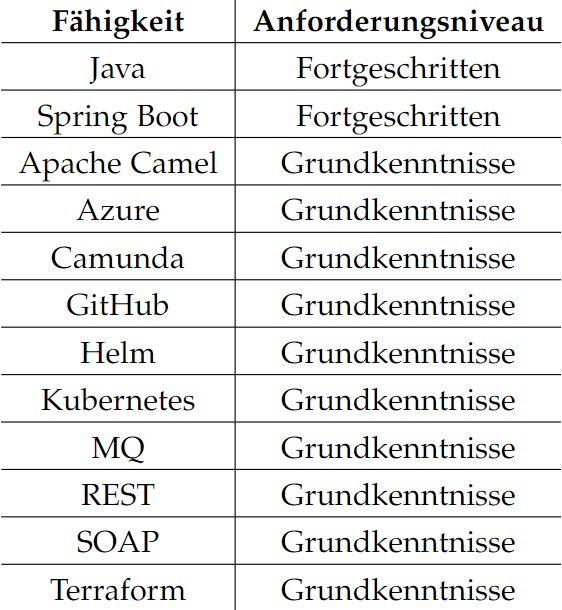
\includegraphics[width=0.5\textwidth]{gfx/projekt-1.png}\label{fig:methodik:abb2:1}}
    \subfloat[Projekt 2]{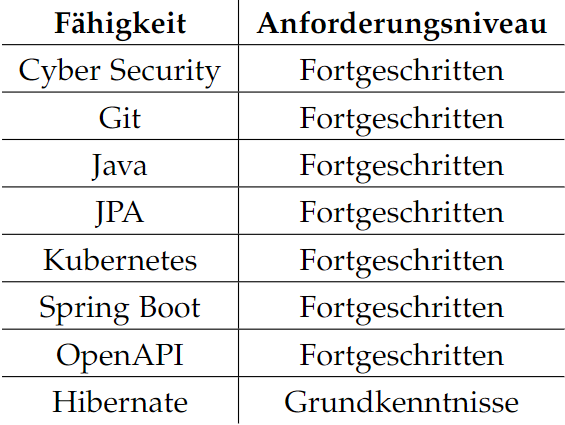
\includegraphics[width=0.5\textwidth]{gfx/projekt-2.png}\label{fig:methodik:abb2:2}}\\
    \subfloat[Projekt 3]{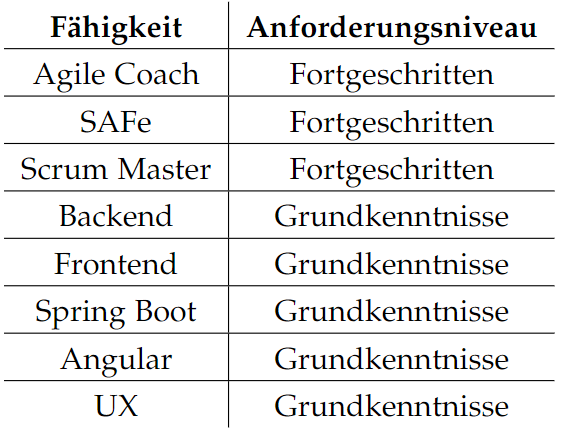
\includegraphics[width=0.5\textwidth]{gfx/projekt-3.png}\label{fig:methodik:abb2:3}}
    \subfloat[Projekt 4]{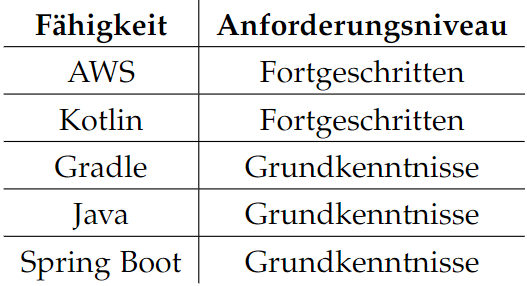
\includegraphics[width=0.5\textwidth]{gfx/projekt-4.png}\label{fig:methodik:abb2:4}}\\
    \subfloat[Projekt 5]{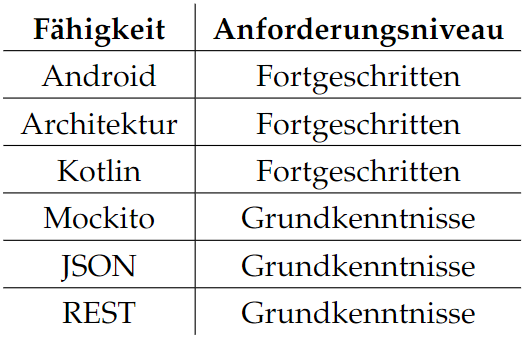
\includegraphics[width=0.5\textwidth]{gfx/projekt-5.png}\label{fig:methodik:abb2:5}}\\
\caption[Beispielprojekte der Fallstudie]{Beispielprojekte der Fallstudie}
  \label{fig:methodik:abb2}
\end{figure}

Für jede Fähigkeit eines Projekts ist ein angefordertes Niveau angegeben, welches in dem Projekt gefragt ist.
Tabelle \ref{tab:methodik:tab1} stellt eine Beschreibung der Kenntnisse dar, die von den Fähigkeiten eines Mitarbeitenden entsprechend des angeforderten Niveaus erwartet wurden.

\begin{table}[htbp]
    \begin{center}
    \begin{tabular}{c|p{3.5in}}
    {\textbf{Anforderungsniveau}} & {\textbf{Beschreibung}}\\
    \hline
	Grundkenntnisse & Kenntnisse entsprechen mindestens einer der Stufen "Ich habe Grundkenntnisse", "Ich habe es schon in einem Projekt eingesetzt" oder "Ich habe es in einem Projekt eingeführt" \\
    \hline
    Fortgeschritten & Kenntnisse entsprechen mindestens einer der Stufen "Ich habe Kollegen geholfen es einzusetzen", "Ich habe eine Schulung zu dem Thema gehalten" oder "Ich habe auf Konferenzen zu dem Thema Vorträge gehalten" \\
    \end{tabular}
    \end{center}
    \caption[Beschreibung des Kenntnisstands eines Mitarbeitenden je Anforderungsniveau]{Beschreibung des Kenntnisstands eines Mitarbeitenden je Anforderungsniveau}
	\label{tab:methodik:tab1}
\end{table}

\subsection{Datenerhebung}
In der zweiten Stufe wurden die benötigten Daten erhoben.
Die Erhebung der Daten erfolgte anhand von zwei separaten Befragungen.
Die erste Befragung wurde unter Mitarbeitenden des Unternehmens durchgeführt.
Die zweite Befragung erfolgte unter den Managern des Unternehmens.
Die Befragungen wurden unabhängig von dem entwickelten Algorithmus gestaltet.
Dadurch ist eine Reproduzierbarkeit der Ergebnisse und deren Vergleichbarkeit mit Ergebnissen alternativer Algorithmen möglich.

\subsubsection{Befragung der Mitarbeitenden}
Die Befragung unter den Mitarbeitenden hatte zwei Erkenntnisse zum Ziel.
Zum einen sollte die Umfrage Auskunft über die Fähigkeiten und Präferenzen eines befragten Mitarbeitenden liefern.
Zum anderen sollte über die Umfrage die Zufriedenheit eines Mitarbeitenden mit den jeweiligen Beispielprojekten aus Tabelle \ref{fig:methodik:abb2} erhoben werden.

Für die Erhebung der Fähigkeiten und Präferenzen wurden die Mitarbeitenden in der Umfrage gebeten, ihr Kenntnisniveau für jede der insgesamt 31 unterschiedlichen Fähigkeiten der Beispielprojekte anzugeben.
Hierfür mussten die Mitarbeitenden ihr Kenntnisniveau auf einer Likert-Skala angeben.
Die Likert-Skala umfasste die Optionen "Keine Kenntnisse", "Grundkenntnisse" und "Fortgeschritten".
Die Optionen "Grundkenntnisse" und "Fortgeschritten" der Skala wurden entsprechend der Skala des Anforderungsniveaus der Fähigkeiten der Beispielprojekte gewählt (Vgl. Tabelle \ref{tab:methodik:tab1}).
Zusätzlich zu den Kenntnisniveaus "Grundkenntnisse" und "Fortgeschritten" konnten die Mitarbeitenden darüber hinaus über die Option "Keine Kenntnisse" angeben, wenn sie in einer Fähigkeit keine Kenntnisse beherrschten.
Abbildung \ref{fig:methodik:abb2} stellt einen Auszug aus der Umfrage zur Erhebung der Fähigkeiten eines Mitarbeitenden dar.

\begin{figure}[H]
    \centering
	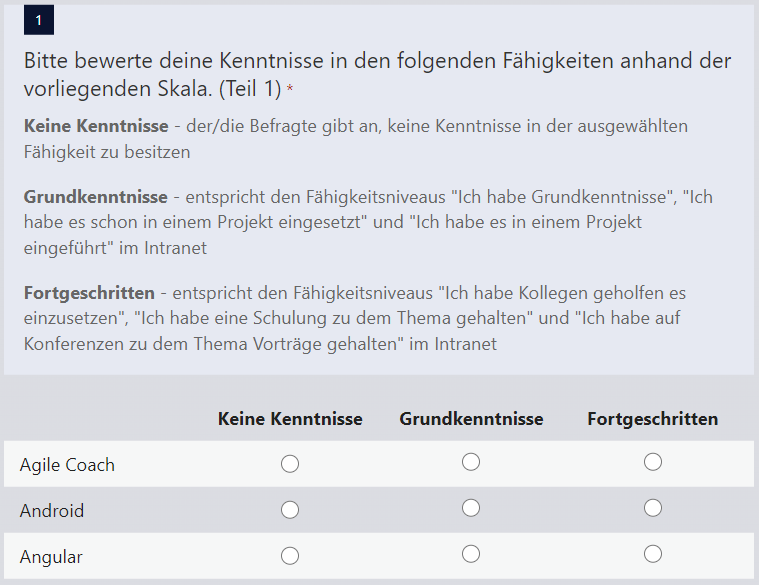
\includegraphics[width=1\textwidth]{gfx/befragung-faehigkeiten.png}
	\caption[Auszug aus der Befragung der Mitarbeitenden zu ihren Fähigkeiten]{Auszug aus der Befragung der Mitarbeitenden zu ihren Fähigkeiten}
	\label{fig:methodik:abb3}
\end{figure}

% Hier erwähnen, dass jeweils zu 31 Fähigkeiten das Kenntnisniveau und Präferenz abgegeben werden musste.
% 1. Mitarbeiter befragen nach Selbsteintschätzung der Fähigkeiten in Anlehnung an Intranet (da im Intranet nur z.T. vollständig), sowie Präferenzen (pos. und neg.)
% Zusätzlich: Bewertung der zufriedenheit eines MA bei Zuteilung zu den verschiedenen Dummy-Projekten
% Erklärung für Auswhal der Skalen

\subsubsection{Befragung der Projektmanager}
% 2. Bewertung der erwarteten Arbeitsleistung von Mitarbeitern unter Berücksichtigung ihrer Fähigkeiten und Präferenzen in den versch. Dummy-Projekten
% Hier ist ein Teil dese Outputs (Präferenzen und Skills) der 1. Befragung der Input dieser Befragung
% Erklärung für Auswahl der Skalen

Zum einen sollten in dessen Rahmen die Fähigkeiten und Präferenzen der befragten Mitarbeitenden erhoben werden.
Zum anderen wurde deren Zufriedenheit mit den jeweiligen Beispielprojekten aus Tabelle \ref{fig:methodik:abb2} ermittelt.

Die zweite Befragung erfolgte unter Managern des Unternehmens und galt der Ermittlung der zu erwarteten Arbeitsleistung der Mitarbeitenden in den jeweiligen Beispielprojekten.

In der dritten Stufe erfolgte die Gestaltung des Empfehlungssystems.
Dieses sollte in der Lage sein, aus einer Menge an zu Verfügung stehenden Mitarbeitenden die fünf passensten Mitarbeitenden anhand eines unilateralen und anhand eines bilateralen Algorithmus zu empfehlen.

Die letzte Stufe umfasste die Evaluation der Algorithmen.


Hierfür wurden im Rahmen zweier separater Befragungen Fähigkeiten, Präferenzen, Zufriedenheit der Mitarbeitenden und erwarteter Arbeitsleistung von Mitarbeitenden erhoben.
Die Erhebung der Daten erfolgte anhand von zwei separaten Befragungen.
Die erste Befragung wurde unter den Mitarbeitenden des Unternehmens durchgeführt.
Zum einen sollten in dessen Rahmen die Fähigkeiten und Präferenzen der Mitarbeitenden erhoben werden.
Zum anderen wurden deren Zufriedenheit m

% Art der Methodik
% quantitative Forschung in Form einer Befragung

% \subsection{Bestimmung der Stichprobe}
% MA im JES-Team, Manager, angeben wie viele kontakiert wurden (Anzahl MA, Anzahl Manager)

% 2 separate Befragungen
% Befragung ist unabhängig von dem gewählten algorithmus -> dadurch reproduzierbarkeit und vergleichbarkeit möglich
% Aufteilen der Daten in Trainings- und Testdaten
% Nutzen der Trainingsdaten, um Gewichte des bilateralen Algorithmus zu lernen
% Vergleich des entwickelten bilateralen Algorithmus mit einer unilateralen Variante anhand der Testdaten

\subsection{Gestaltung des Empfehlungssystems}
Für die Gestalung des Algorithmus wurden die im Rahmen der Befragungen erhobenen Daten in Trainings- und Testdaten unterteilt.

% \subsection{Aggregation}
% Beispielrechnung in Anhang?
% Begründung Auswahl der Kombination der Präferernzen
% Kein harmonisches Mittel, da teilen durch 0 nicht möglich. Da aber MA durchaus fähigkeiten nicht besitzen kommt das häufig vor (man könnte als abhilfe einen Default von 0,000001 setzen o.ä.)
% Berücksichtigung negativer Präferenzen in Anlehnung an: S. 231, file://wsl%24/Ubuntu/home/masc6/Projects/masterarbeit/literatur/recsys%202022%20modeling%20two%20way%20selection%20preference%20for%20person%20job%20fit.pdf

% \subsection{Gewichtung}
% Ermitteln der Gewichte: alpha so wählen, dass Endergebnis möglichst optimal -> bedeutet für uns: zufriedene und leistungsfähige Mitarbeiter werden empfohlen -> erscheinen oben im Ranking
% Ziel: Gegeben einer Funktion f, welches von ein oder mehreren Input-Variablen abhängt, finden der Ausprägungen der Input-Variablen, für die f minimal wird. Obacht: f umfasst hier mehr als nur rws, da auch das ranking danach miteinbezogen wird -> zu minimieren ist die Summe der Ränge der zufriedenen und Leistungsfähigen MA über alle Projekte hinweg
% Hier: mithilfe des Brent Algorithmus in anlehnung an die verwandte Arbeit von \textcite[S. 131ff.]{kleinerman:2:inproceedings}
% Nach https://e-maxx.ru/bookz/files/numerical_recipes.pdf S. 489 gibt es keinen perfekten Optimierungs-Algorithmus -> daher ist es grundsätzlih ratsam, verschiedene Techniken auszuprobieren und zu vergleichen.
% Was macht der Brent Algorithmus?: % https://users.wpi.edu/~walker/MA3257/HANDOUTS/brents_algm.pdf

% \begin{itemize}
% 	\item In Essenz einfach eine Strategie für das Finden von lokalen Minima ohne Ableitung, indem sich von einem Intervall iterativ an ein Minima angenähert wird, entweder über GSS oder über SPI % file://wsl%24/Ubuntu/home/masc6/Projects/masterarbeit/literatur/Minimization%20or%20Maximization%20of%20Functions.pdf
% 	\item Unterscheiden zw. Brent Methode für root search und Brent-Methode für Minimasuche ohne Derivate (Ableitung)
% 	\item Kombination von successive parabolic interpolation (schnell) und golden-section search (garantiertes finden von Minimum) % für Erklärung siehe video hier: https://www.youtube.com/watch?v=BQm7uTYC0sg
% \end{itemize}

% Lösung über Python Skript unter Einsatz der scipy-Bibliothek (siehe Anhang).
% minimize_scalar function für das Finden von Minima einer skalaren Funktion (output eines einzelnen Wertes) mit einer Variablen (in unserem Fall alpha), deren default Methode brent ist
% Angeben eines Intervalls (hier: zwischen 0 und 1)
% Beschreibung des Algorithmus in anlehung an file://wsl%24/Ubuntu/home/masc6/Projects/masterarbeit/literatur/Minimization%20or%20Maximization%20of%20Functions.pdf ggf. in den Anhang?

% \section{Aufbau des Empfehlungssystems}
% Microservice-Architektur -> Empfehlungs-komponente (Rankings)

% \begin{figure}[H]
%     \centering
% 	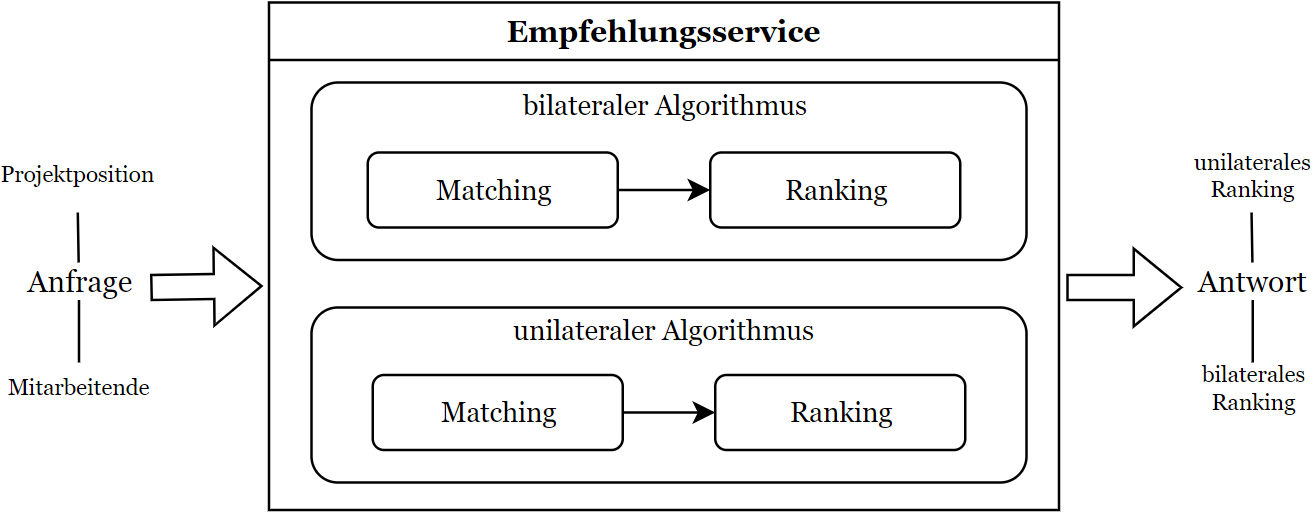
\includegraphics[width=1.0\textwidth]{gfx/empfehlungsservice.png}
% 	\caption[Aufbau des bilateralen Empfehlungssystems]{Aufbau des bilateralen Empfehlungssystems}
% 	\label{fig:algorithmus:abb1}
% \end{figure}

% Begründung für SVR: S: 30, file://wsl%24/Ubuntu/home/masc6/Projects/masterarbeit/literatur/Criteria%20Chains%20A%20Novel%20Multi-Criteria%20Recommendation.pdf

\subsection{Datenauswertung}

\shorthandon{"}